\documentclass[10pt,a4paper]{article}
\usepackage{libertine}
\setmonofont{Inconsolatazi4}[Extension=.otf,UprightFont=*-Regular,BoldFont=*-Bold,Scale=MatchLowercase]
\usepackage{microtype}
\usepackage[margin=19mm,headheight=14pt]{geometry}
\usepackage{graphicx,xcolor,booktabs,tabularx,array,enumitem}
\usepackage{tikz}
\usetikzlibrary{arrows.meta,positioning,fit,backgrounds}
\usepackage{tcolorbox,fancyhdr,titlesec,listings}
\usepackage[hidelinks]{hyperref}
\graphicspath{{assets/}{./}}
\definecolor{Ink}{HTML}{15243A}
\definecolor{Blue}{HTML}{245DE9}
\definecolor{Teal}{HTML}{087F8C}
\definecolor{Muted}{HTML}{5E6D82}
\definecolor{Pale}{HTML}{F2F6FC}
\definecolor{Line}{HTML}{D8E2F0}
\renewcommand{\familydefault}{\rmdefault}
\color{Ink}
\setlength{\parindent}{0pt}
\setlength{\parskip}{5pt}
\setlength{\emergencystretch}{2em}
\setlength{\tabcolsep}{5pt}
\renewcommand{\arraystretch}{1.2}
\setlist[itemize]{leftmargin=*,nosep,topsep=3pt}
\setlist[enumerate]{leftmargin=*,nosep,topsep=3pt}
\titleformat{\section}{\sffamily\Large\bfseries\color{Blue}}{\thesection}{0.65em}{}
\titleformat{\subsection}{\sffamily\normalsize\bfseries}{\thesubsection}{0.65em}{}
\titlespacing*{\section}{0pt}{9pt}{7pt}
\titlespacing*{\subsection}{0pt}{7pt}{3pt}
\pagestyle{fancy}
\fancyhf{}
\fancyhead[L]{\small\textcolor{Muted}{CONTEXTLEDGER}}
\fancyhead[R]{\small\textcolor{Muted}{FINTECH / INTERNAL BRAIN}}
\fancyfoot[L]{\footnotesize\textcolor{Muted}{Submission report \textbullet\ 15 October 2026}}
\fancyfoot[R]{\footnotesize\thepage}
\renewcommand{\headrulewidth}{0.3pt}
\newcolumntype{Y}{>{\raggedright\arraybackslash}X}
\newcommand{\hb}[1]{{\footnotesize\textcolor{Muted}{[Handbook, p.~#1]}}}
\newcommand{\evidence}[1]{{\footnotesize\textcolor{Muted}{[Evidence #1]}}}
\newcommand{\smalllabel}[1]{{\small\bfseries\color{Teal}#1}}
\newtcolorbox{noteBox}{colback=Pale,colframe=Line,boxrule=0.5pt,arc=2mm,left=8pt,right=8pt,top=6pt,bottom=6pt}
\lstset{basicstyle=\ttfamily\footnotesize,breaklines=true,columns=fullflexible,keepspaces=true,showstringspaces=false,backgroundcolor=\color{Pale},frame=single,rulecolor=\color{Line},xleftmargin=0pt,xrightmargin=0pt}

\begin{document}
\thispagestyle{empty}
\smalllabel{TENCENT CLOUD AI CAN DO IT 2026 \quad / \quad FINTECH TRACK -- ASPIRE}
\vspace{9mm}

{\fontsize{38}{42}\selectfont\bfseries ContextLedger\par}
\vspace{3mm}
{\Large Permission-aware enterprise knowledge,\par grounded in current evidence.\par}
\vspace{6mm}
\begin{noteBox}
\textbf{Selected case study}\par
The Internal Brain -- Building a Context-Aware Enterprise Knowledge System with RBAC, Security Logging \& Audit Trail. \hb{15}
\end{noteBox}
\vspace{4mm}
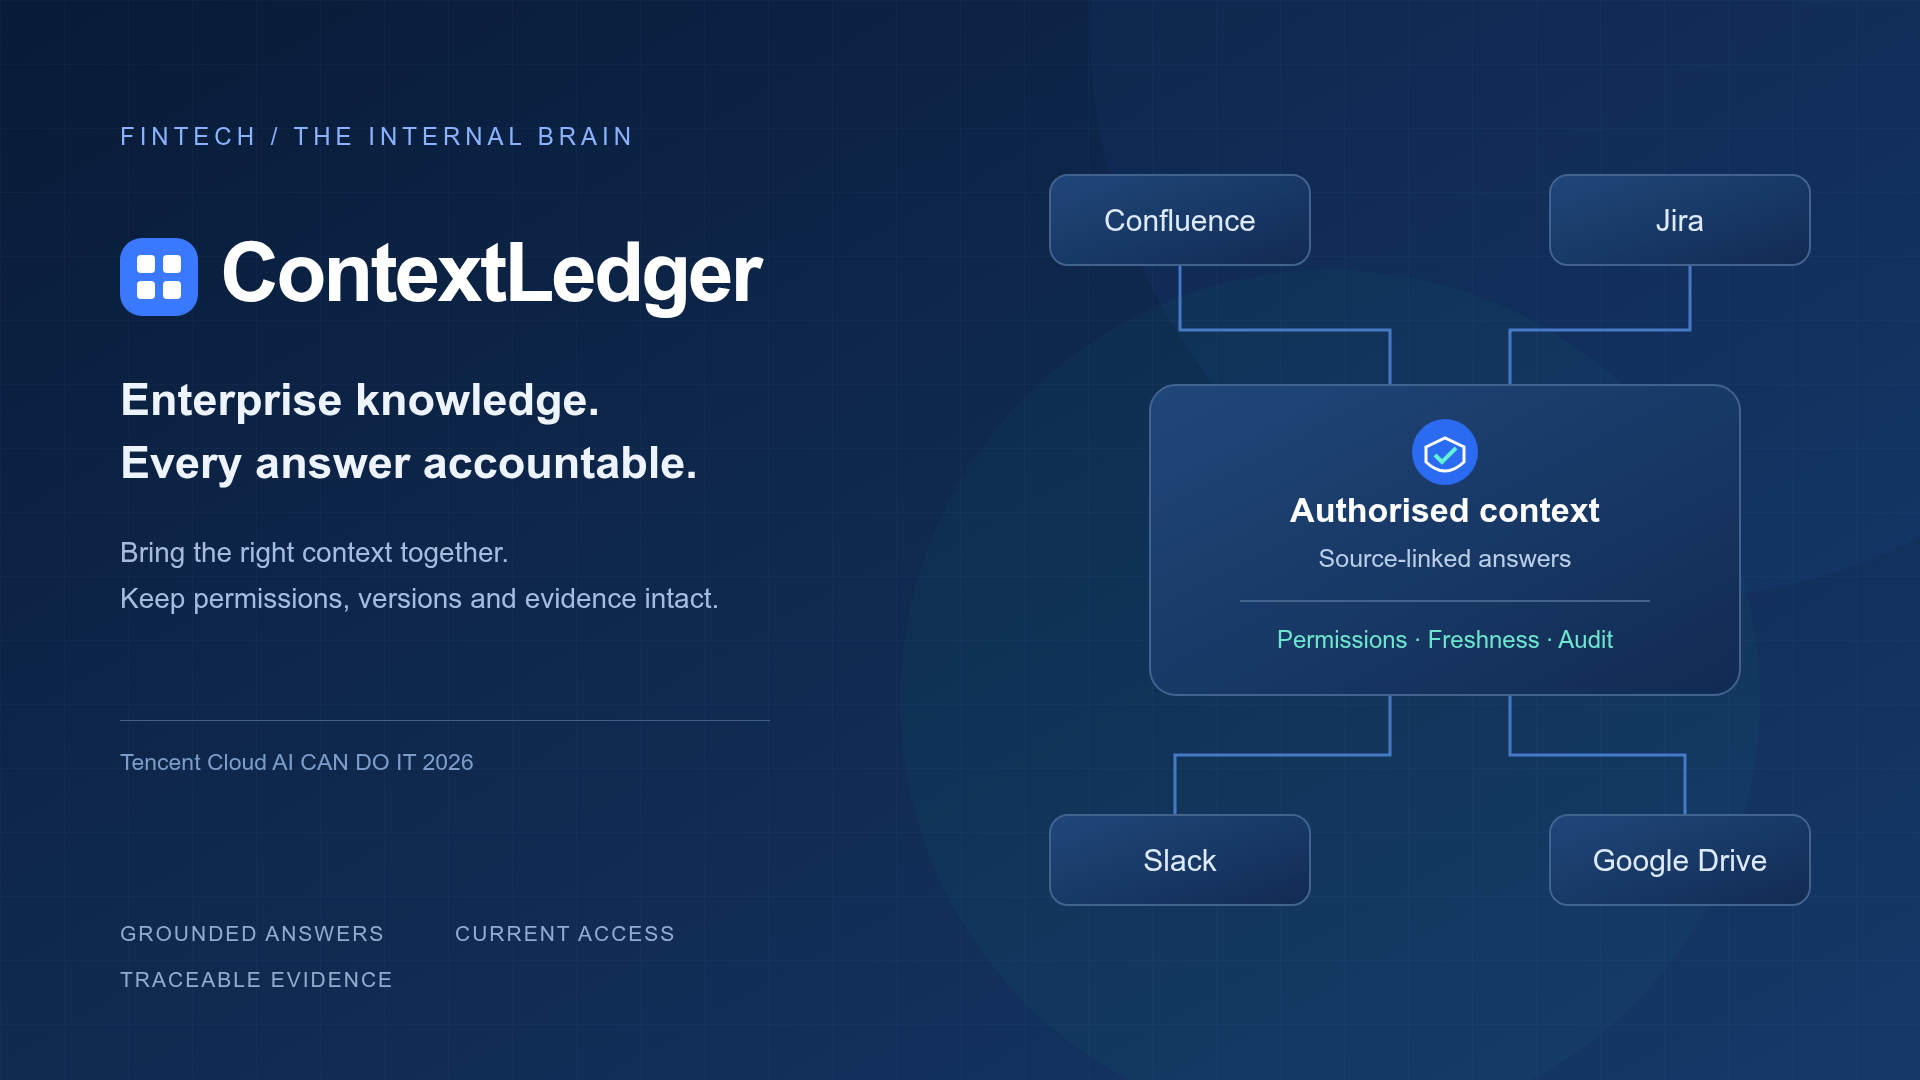
\includegraphics[width=\linewidth]{cover.png}
\vspace{4mm}
\smalllabel{SHORT BLURB -- 8 WORDS}
\par Enterprise answers with permissions, freshness, and traceable evidence.

\subsection*{Project at a glance}
An employee investigating an incident may need a Jira ticket, a Slack discussion and a current runbook to answer the same question. ContextLedger searches the records that employee is allowed to read, returns an answer with source links and logs the request. For decisions or incident history, the internal Decision Radar tool can retrieve further authorised records and separate recorded status from reported claims.

The prototype covers the Handbook's five scenarios with controlled examples. Recorded tests cover retrieval, updates, revocation, real-model answers and browser interactions. The current version uses imported or synthetic records. Live integration with all four platforms and enterprise authentication still require validation.

\vfill
{\small\color{Muted}Prepared by the ContextLedger team \quad | \quad 15 October 2026\par
Report basis: Handbook pp.~14--20 and 37; repository baseline \texttt{952881f}; dated experiment records.}

\clearpage
\section{Project Overview}
\subsection{Target scenarios, users and value proposition}
The Handbook starts with an on-call engineer trying to piece together tickets, discussions, runbooks and postmortems during an incident. Those records sit in four platforms, each with its own permissions and update times. ContextLedger brings the relevant records into the same answer while keeping access limited to what the employee is authorised to read. \hb{15--17}

\begin{tabularx}{\linewidth}{@{}>{\raggedright\arraybackslash}p{29mm}YY@{}}
\toprule
\textbf{Target user} & \textbf{Handbook-grounded task} & \textbf{Value offered} \\
\midrule
On-call and backend engineers & Reconstruct a payment outage, find follow-up tickets, or identify migration blockers in Slack. & Read one evidence-backed account with links to the relevant technical records. \\
Project and operations staff & Follow a project or approval across tickets, discussions and documents. & Distinguish a proposal, an approval and an effective change before acting. \\
Junior staff and contractors & Ask ordinary questions within a narrower access scope. & Get useful authorised evidence without exposing restricted content or its existence. \\
Compliance officers and administrators & Reconstruct what a user asked, accessed and received over a time period. & Inspect attributable events and verify the audit chain under a separate access boundary. \\
\bottomrule
\end{tabularx}

The challenge explicitly names engineers, junior employees, contractors, administrators and compliance officers. We also include project and operations staff because the questions about project status and decisions apply to their work. \hb{16--19}

\section{Real-World Scenario Insights}
\subsection{Where the pain points come from}
Company A in the Handbook has over 50 Confluence spaces and 12,000 pages, over 30 Jira projects, over 200 Slack channels, and shared and personal Google Drives. Employees must find the relevant records and work out how they relate. The Handbook estimates that this search and the resulting questions to colleagues take about 30\% of the workweek. These figures describe the challenge scenario; we have not measured employee search time or savings from ContextLedger. \hb{16}

\begin{tabularx}{\linewidth}{@{}>{\raggedright\arraybackslash}p{35mm}YY@{}}
\toprule
\textbf{Core problem} & \textbf{Business consequence} & \textbf{Design response} \\
\midrule
Fragmented context & A ticket alone omits the discussion, decision document or current runbook. & Assemble cross-source evidence and preserve source links. \\
Different access models & A shared assistant could disclose private channels, restricted pages or secured issues. & Preserve source ACL meaning and enforce current identity before model context assembly. \\
Changing facts and access & An obsolete runbook or a revoked permission can still influence an answer. & Track versions and publication state; block stale evidence and recheck permissions before delivery. \\
Unsupported synthesis & A merged PR, a deployment report and operational recovery can be wrongly treated as the same event. & Separate recorded states, claims and unresolved conflicts; show uncertainty and citations. \\
Missing accountability & Compliance cannot reconstruct who saw what or detect altered logs. & Record attributable requests, evidence and answers in a queryable, tamper-evident chain. \\
\bottomrule
\end{tabularx}

The aim is to reduce the work needed to reconstruct an incident or decision without widening access to sensitive records. Source links and audit events let employees and compliance staff check how an answer was reached. The evaluation below shows what has been tested; workplace time savings still need measurement.

\clearpage
\section{Worked Examples for the Five Required Scenarios}
Each example below addresses a scenario required by the Handbook. The business names and amounts are synthetic test fixtures, with no Aspire customer or production data. \hb{18--19}

\subsection{1. Unified natural-language query}
\textbf{Question:} Is QuartzPay's proposed CNY~60,000 daily transfer limit active?

\textbf{Evidence and response:} The Confluence proposal gives the amount. The Jira approval record says it is pending and has not taken effect. The answer cites both records and explains that the current active limit is unknown from this evidence. A CedarPay counterpart records an approved, effective CNY~70,000 limit and provides a positive control. Both require the cross-platform evidence assembly described in the Handbook's Jira-plus-Slack migration example. \evidence{E1}

\subsection{2. Data freshness}
\textbf{Question:} What is TracePay's current daily transfer limit?

\textbf{Action and observed outcome:} An administrator changes the fixture from CNY~50,000 to CNY~120,000 through the update API. A persistent job updates canonical text, keyword entries and affected vectors before publishing a checked generation. Once publication is ready, keyword, vector and hybrid answers use CNY~120,000 and the new evidence hash. Six before/after answer checks passed. \evidence{E1}

This check starts after publication is ready. The Handbook requires source changes to reach answers within a predictable window of minutes to approximately one hour, which this check does not measure. A separate online replay includes requests made during updates and keeps unavailable and failed requests in its denominators. \hb{18}

\subsection{3. Permission enforcement without a metadata side-channel}
\textbf{Action:} Ask the same protected question as an employee without the relevant source binding, or ask about an unknown entity.

\textbf{Observed outcome:} The service returns an insufficient-evidence response with no evidence or citations and does not call the answer model. It reveals neither hidden titles and document identifiers nor whether a restricted record exists. Nine unknown/unauthorised observations passed in the 42-observation chat regression. \evidence{E1}

\subsection{4. Live permission change handling}
\textbf{Action:} First retrieve authorised material; then revoke that employee's business access while keeping the account and session valid. Repeat the question and try opening an old source reference.

\textbf{Observed outcome:} Subsequent answers contain no protected evidence, and old-document access is denied. Three post-revocation chat observations passed without answer-model calls. The controlled permission suite also changes access during retrieval and generation. The service discards the response when its permission snapshot is no longer valid. These checks cover system-local revocation; automatic discovery of source-platform permission changes is still to be validated. \evidence{E1, E2}

\subsection{5. Audit inquiry}
\textbf{Question:} What did this user access last week, and what evidence supported the answers?

\textbf{Workflow:} An administrator or compliance officer searches the protected audit interface by user, document, request or time range. The results include timestamps, retrieved document IDs, evidence versions, authorisation decisions and answers. The inquiry is logged, and details outside the auditor's current business access are redacted. The chat and controlled permission runs retain valid hash chains. External immutable anchoring and complete enterprise-wide event coverage still need validation. \evidence{E1, E2}

\clearpage
\section{Three Product Innovations}
The three features work together on one question: \emph{Has SG Batch Payments v2.3 recovered, and can we tell customers that service is normal?} Decision Radar assembles the business context, Security Lens controls who can use it, and Evidence Passport lets the reader inspect its sources. The incident below is a fictional demo.

\subsection{Decision Radar: follow how a business conclusion forms}
A relevant message is a starting point. To decide whether a service has recovered, an employee also needs the incident state and the runbook's confirmation conditions. Radar brings these records together within the employee's current access scope. The answer separates recorded facts from unresolved conditions.

\begin{tabularx}{\linewidth}{@{}>{\raggedright\arraybackslash}p{34mm}YY@{}}
\toprule
\textbf{Capability} & \textbf{What the employee sees} & \textbf{Why it helps} \\
\midrule
Decision Timeline & Related discussions, tickets and document revisions organised by recorded event time; unknown times stay unknown. & Follow a proposal, confirmation, change or withdrawal across platforms. \\
Conflict Radar & Differing source states, their references and unresolved confirmation conditions. & Avoid treating a recovery message as proof that monitoring criteria have been met. \\
Answer Replay & The recorded question, answer, evidence versions, permission snapshot and model diagnostics, where retained and currently visible. & Reconstruct the basis of a past response for review. \\
\bottomrule
\end{tabularx}

\begin{noteBox}
\textbf{Illustrative demo sequence.} At 09:40, a Slack message reports recovery. At 09:47, the Jira incident remains open. At 09:50, a runbook record states that monitoring validation is required before formal confirmation. The useful result is \emph{``Full recovery is not yet confirmed: check monitoring validation and reconcile the incident state.''} An open ticket could reflect a delayed update; it does not, by itself, prove an outage. 
\end{noteBox}

The prototype supports bounded internal evidence expansion, revision references, event candidates and source-difference reporting. The new frontend presents a timeline and a pending/confirmed summary. The summary describes the selected records; live service health requires operational evidence. Complete cross-source authority rules and semantic conflict detection remain unvalidated. Answer Replay uses the audit record; it does not deterministically rerun a historical model or restore revoked access.

\subsection{Security Lens: make permission changes visible}
An administrator selects a demo employee, removes a source binding or applies a restriction, then repeats the search and tries opening an earlier citation. The expected change is concrete: evidence outside the new scope stops reaching search results, model input, answers and source views. An in-flight response is discarded if its permission snapshot changes. The controlled permission results are reported separately in the evaluation section.

The new frontend provides the administrator interaction and shows the recorded change. This covers system-local permissions; discovery of changes in live source platforms still needs validation. Employee refusals reveal no restricted titles or document existence. Administrative and compliance details require their own authorisation, and an administrator role alone does not grant business-document access.

\subsection{Evidence Passport: inspect the basis of an answer}
Opening a citation shows the source text, platform, document version, index time and current access basis. Technical details retain the content hash and provenance where available. A reader can distinguish a formal approval record from a discussion proposing the same change, and can check which record supports the answer.

The current Passport is a source-inspection view. Automatic claim-by-claim support mapping remains future work: valid citation IDs and authorised sources do not establish that every sentence follows from them. No confidence score is assigned. Missing evidence is a gap in the bounded selection, rather than proof that no such record exists.

\clearpage
\section{Comprehensive Solution Design}
\subsection{Business workflow and technical architecture}
When an employee asks a question, the application checks current identity and permitted source principals. Search returns authorised evidence for the answer stage, and the employee can open the source text. Separate administrator operations manage permissions and document updates. Compliance users access request history through the protected audit interface.

\begin{center}
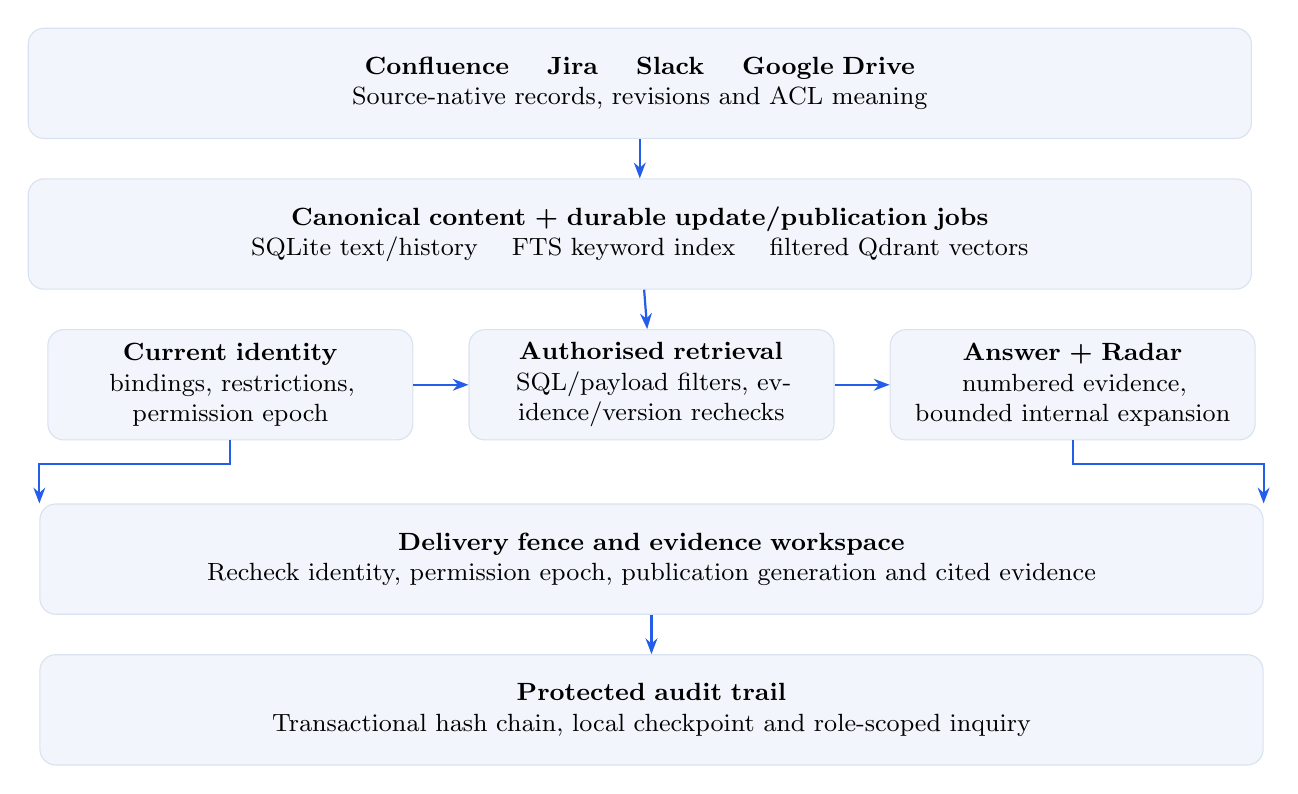
\begin{tikzpicture}[node distance=5mm and 7mm,box/.style={draw=Line,rounded corners=2mm,fill=Pale,align=center,text width=44mm,minimum height=14mm,font=\small},wide/.style={box,text width=153mm},arr/.style={-{Stealth[length=2mm]},thick,draw=Blue}]
\node[wide] (sources) {\textbf{Confluence \quad Jira \quad Slack \quad Google Drive}\\Source-native records, revisions and ACL meaning};
\node[wide,below=of sources] (stores) {\textbf{Canonical content + durable update/publication jobs}\\SQLite text/history \quad FTS keyword index \quad filtered Qdrant vectors};
\node[box,below=of stores,xshift=-52mm] (identity) {\textbf{Current identity}\\bindings, restrictions, permission epoch};
\node[box,right=of identity] (retrieve) {\textbf{Authorised retrieval}\\SQL/payload filters, evidence/version rechecks};
\node[box,right=of retrieve] (model) {\textbf{Answer + Radar}\\numbered evidence, bounded internal expansion};
\node[wide,below=8mm of retrieve] (delivery) {\textbf{Delivery fence and evidence workspace}\\Recheck identity, permission epoch, publication generation and cited evidence};
\node[wide,below=of delivery] (audit) {\textbf{Protected audit trail}\\Transactional hash chain, local checkpoint and role-scoped inquiry};
\draw[arr] (sources)--(stores);
\draw[arr] (stores)--(retrieve);
\draw[arr] (identity)--(retrieve);
\draw[arr] (retrieve)--(model);
\draw[arr] (model.south)--++(0,-3mm)-|(delivery.north east);
\draw[arr] (identity.south)--++(0,-3mm)-|(delivery.north west);
\draw[arr] (delivery)--(audit);
\end{tikzpicture}
\end{center}
{\footnotesize\textcolor{Muted}{Figure 1. Request and publication boundaries in the assessed baseline. The source layer uses imported records and controlled updates; live connectors have not been validated.}}

\subsection{How the boundaries are enforced}
\begin{itemize}
\item \textbf{Access.} Source ACL authorisation requires an explicitly bound source identity and must satisfy current local restrictions. Being an administrator does not grant access to every business document. FTS uses SQL authorisation predicates, and Qdrant uses payload filters. Returned records are checked against canonical content.
\item \textbf{Freshness.} Content versions, hashes, indexed metadata and publication generations must agree before delivery. Pending, failed or inconsistent publication blocks the response. Durable updates modify the affected document and vectors while preserving historical content. Index rebuilds retain the identity and audit stores.
\item \textbf{Model boundary.} Only authorised evidence enters the prompt. Radar uses server-side identity and scope, with one tool invocation, up to two expansion rounds and explicit material/time budgets. Historical evidence is labelled so it is not presented as current state.
\item \textbf{Delivery and audit.} The service checks permissions and versions around model calls and before the HTTP response. Audit append is transactional and hash-linked; browser responses use no-store caching. A later revocation cannot recall information already delivered.
\end{itemize}
\evidence{E3}

\clearpage
\subsection{How prompts drive AI generation}
The prompt keeps the original question, caller context and numbered authorised evidence in separate fields. Source text is treated as untrusted data. The main answer prompt asks for a direct answer in the user's language, with citations beside factual claims and an explanation of any gaps or conflicts. The result must use the specified JSON structure. Prompt versions are recorded for reproducibility; access rights are enforced by code. \evidence{E3}

\begin{tabularx}{\linewidth}{@{}>{\raggedright\arraybackslash}p{29mm}YY@{}}
\toprule
\textbf{Stage} & \textbf{Prompt role} & \textbf{Deterministic control} \\
\midrule
Optional query planning & Suggest bounded search branches or ask for clarification while keeping the original question. & Validate branch schema and budget; every branch uses current authorised scope. \\
Answer/tool selection & Answer from sufficient evidence, or request history, relationship or status expansion through Radar. & Validate allowed tool arguments and identifiers. The model cannot select identity or permission scope. \\
Radar synthesis & Explain source states, revisions and unresolved differences using expanded authorised evidence. & Shared citation registry, one invocation, bounded expansion and repeated delivery fences. \\
Audit explanation & Explain only the visible, redacted events and cite their event IDs. & Admin/compliance role checks, event filtering, hash-chain verification and access redaction. \\
\bottomrule
\end{tabularx}

\smalllabel{ILLUSTRATIVE INPUT AND OUTPUT -- SYNTHETIC QUARTZPAY EXAMPLE}
\begin{lstlisting}
Input:
original_question: "Is QuartzPay's CNY 60,000 limit active?"
authorised_evidence:
  [1] Confluence: proposed limit is CNY 60,000.
  [2] Jira: approval pending; proposal not yet effective.

Expected output shape:
{"status":"answered",
 "answer":"The CNY 60,000 proposal [1] is still pending
 approval and has not taken effect [2]. The current active
 limit is not recorded in this evidence [2].",
 "citation_ids":[1,2], "uncertainty":"high"}
\end{lstlisting}

An answer can explain a pending decision without implying business approval. When sources conflict, the prompt asks the model to cite both and describe the disagreement. A PR's merged status alone does not show that production recovered. A dated source report is also a claim to be attributed, rather than independent verification.

The service checks output structure, citation identifiers and observed language/format failures. It allows one bounded format repair, then returns a labelled safe fallback if repair fails. A request with zero authorised evidence ends before generation. These checks restrict citations to the supplied evidence; they do not verify sentence-by-sentence factual entailment.

\subsection{Model configuration and evaluation scope}
The 13 October real-chat regression used DeepSeek V3.2 through an OpenAI-compatible endpoint, with 17 synthetic documents and the actual HTTP/Qdrant/audit paths. Earlier freshness experiments tested different models on a narrower single-fact task. We report those scores separately because the tasks differ. Optional planning was disabled in the accepted chat run, so its independent quality benefit remains unmeasured. \evidence{E1, E2}

\clearpage
\section{Business Value and Evaluation}
\subsection{Practical results from the 15 October run}
We tested the frozen prototype at \texttt{952881f} with native MiniLM/Qdrant, controlled updates and permissions, public retrieval questions and real DeepSeek V3.2 answers. The table answers five practical questions about the prototype. Single-request answer timings and fees use 17 synthetic documents and exclude the batch/concurrency trials. \evidence{E7}

\begin{tabularx}{\linewidth}{@{}>{\raggedright\arraybackslash}p{24mm}>{\raggedright\arraybackslash}p{59mm}Y@{}}
\toprule
\textbf{Metric} & \textbf{Measured result} & \textbf{Tested scope} \\
\midrule
Freshness & \textbf{Publication p50: 74 ms; p95: 137 ms.} New-version Recall at 100 ms: 90.74\%; at 250 ms: 100.00\%. & 54 source changes across three runs, against 1,000 background documents. The clock starts at local source release. \\
Permissions & \textbf{False allows: 0/486. False denials: 0/432.} Real in-flight revocations blocked: 3/3. & 918 checks across search, ask and open. Zero observed unauthorized candidate, model-input, evidence or audit IDs. Controlled ACL truth. \\
Recall & \textbf{Hybrid document Recall@10: 66.30\%.} Saved offline ranking refinement: 91.98\%. & Offline Recall score uses 180 fully covered EnterpriseRAG questions. The offline refinement is not enabled in the serving path. \\
Latency & \textbf{p50: 4.74 s; p95: 12.94 s; maximum: 15.03 s.} & 60 sequential English, answerable HTTP requests. Timing includes retrieval, model calls and retries. \\
Model cost & \textbf{Total billed fee: USD 0.014675.} USD 0.000245 per answer passing reviewed checks. & 89 provider calls for the selected 99-request cohort, including retries and three discarded answers. Denied requests make zero model calls. \\
\bottomrule
\end{tabularx}

\subsection{Retrieval detail and corpus coverage}
The offline retrieval run uses the existing token-aware Part A snapshot and executes all 578 public questions once in each mode. The table below scores the 180 EnterpriseRAG questions with all reference documents imported.

\begin{center}
\small
\begin{tabular}{@{}lrrrr@{}}
\toprule
\textbf{Method} & \textbf{Recall@1} & \textbf{Recall@5} & \textbf{Recall@10} & \textbf{Recall@20} \\
\midrule
Keyword & 38.56\% & 53.74\% & 61.19\% & 65.29\% \\
Vector & 34.35\% & 49.12\% & 55.86\% & 60.86\% \\
Hybrid & 43.96\% & 62.04\% & 66.30\% & 72.58\% \\
\bottomrule
\end{tabular}
\end{center}

Of the 500 EnterpriseRAG questions, 290 lack some imported reference evidence and 30 have no reference evidence. Including all 470 questions with references, hybrid Recall@10 is 30.06\%. OrgForge has 78 questions, of which 29 are fully covered; hybrid Recall@10 on those 29 is 9.77\%. These coverage figures explain why the covered-subset score should not be read as recall on every question. Part A does not isolate candidates before ACL filtering; the permission tests above use the integrated filtered service.

The saved ranking refinement reaches 91.98\% on all 180 covered EnterpriseRAG questions and 91.40\% on its reused 160-question validation subset. We independently rescored the saved document IDs; this is an offline result, with no new GPU inference or serving-speed claim. The public questions have already been used for development. \evidence{E8}

\subsection{Answer checks, tokens and limits}
All 60 generated requests use the real model and retrieve and cite their required reference documents with the expected evidence hashes. The original checker passes 58/60 overall. Correcting its recognition of \emph{Chinese Yuan (CNY)} gives 60/60; the two original failures and the revised scores are both retained. These are defined fact/citation checks, rather than full semantic accuracy.

The selected single-request cohort reports 145,386 prompt tokens, 7,188 completion tokens and 121,856 cached prompt tokens. 89/89 completion attempts have observed billed fees. The fee above uses provider billing, with the cost of retries and discarded answers included. Hosting and engineering costs are outside this API-fee measurement.

Source-platform notification delay, real enterprise ACL inheritance, SSO and employee time savings still need validation. The prototype can update a policy, block a revoked account and return cited records at the measured response time and API fee. A short user study should compare manual four-platform search with ContextLedger on the Handbook's incident and approval tasks. \hb{16--19}
\clearpage
\section{User Experience and Remaining Acceptance Work}
The workspace brings the question, answer and sources together. Radar shows the available timeline and source differences; Full answer expands the detailed response. A citation opens its Evidence Passport.

\begin{center}
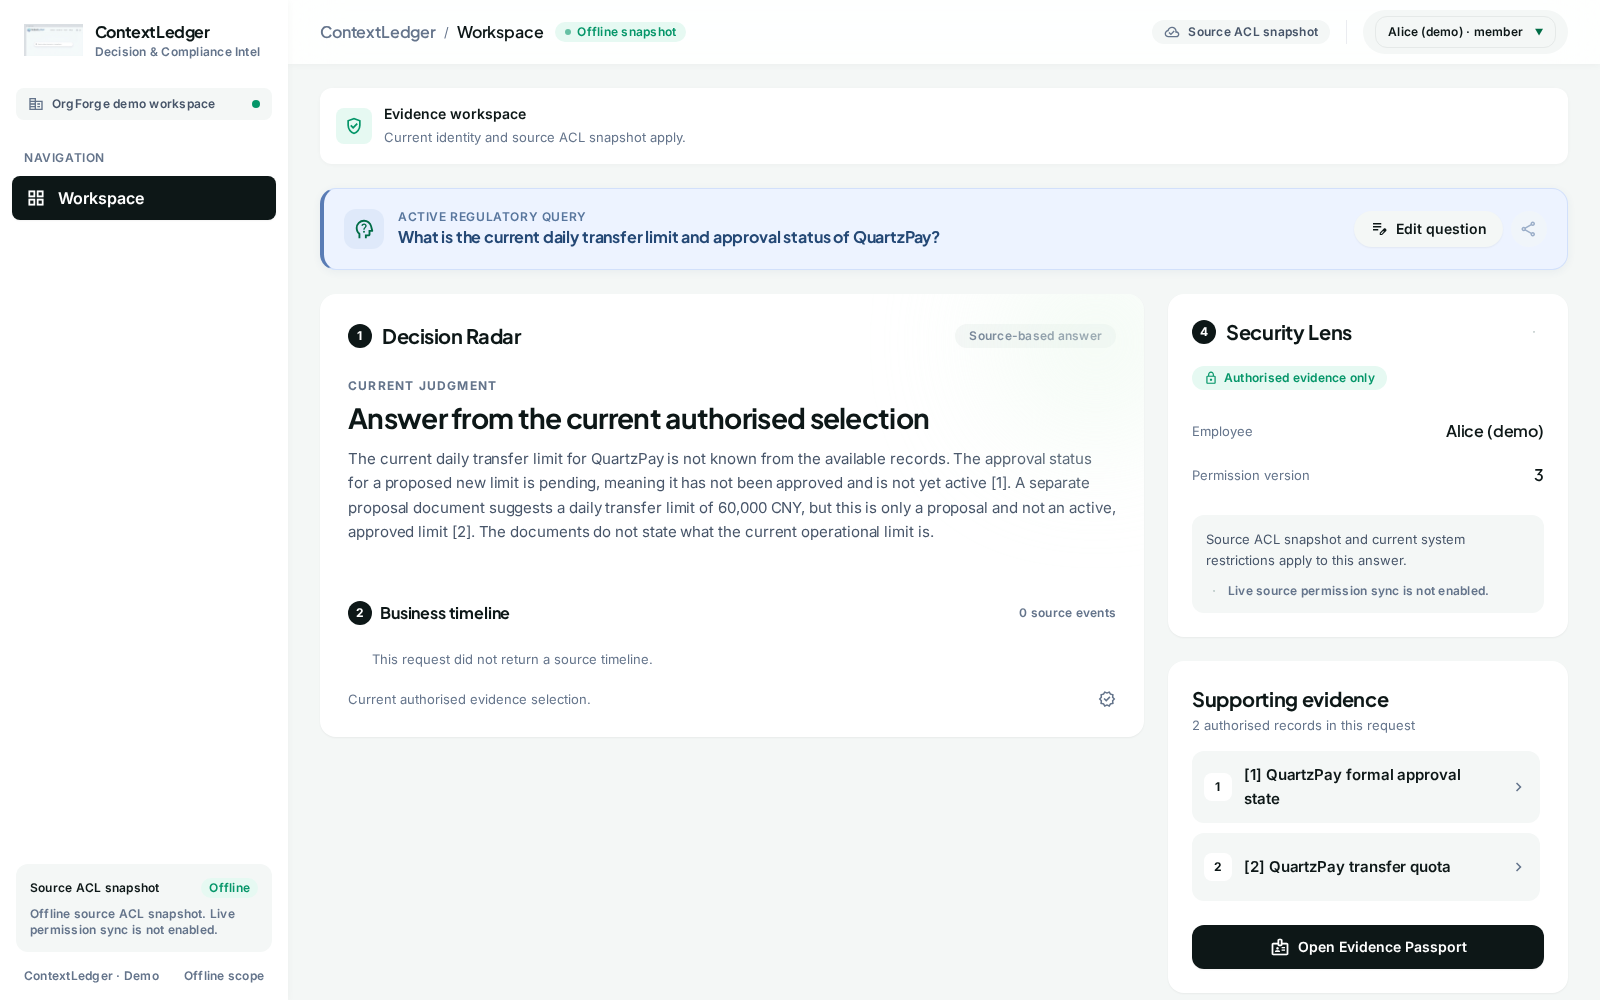
\includegraphics[width=0.96\linewidth]{workspace-latest-en.png}
\end{center}
{\footnotesize\textcolor{Muted}{Figure 2. English frontend build \texttt{b5970553}, captured on 15 October. Recorded API data replays the 13 October QuartzPay answer and citations unchanged. Evaluation results use baseline \texttt{952881f}.}}

\begin{tabularx}{\linewidth}{@{}>{\raggedright\arraybackslash}p{34mm}Y@{}}
\toprule
\textbf{Acceptance boundary} & \textbf{What remains to establish} \\
\midrule
All four live platforms & Verify APIs, pagination, rate limits, native permission meaning and complete configured-source sync with real platform accounts. Imported platform-labelled records do not complete this requirement. \\
Trusted enterprise identity & Replace the isolated fixed-account demo with trusted end-user identity. Browser OIDC is deferred; private network access is not enterprise RBAC. \\
Source freshness/revocation & Measure from the source event to visible, correct answers under a predictable window; validate automatic discovery of source permission changes and source outages. \\
Audit durability/coverage & Add external immutable anchoring and establish meaningful-action and per-document decision coverage at enterprise scale. A local checkpoint alone cannot resist an attacker replacing all local state. \\
Answer quality/latency & Freeze configuration for unseen questions, judge claim support and business-state distinctions, and reduce large-input failures and long response tails without relaxing access or citation checks. \\
\bottomrule
\end{tabularx}

The evaluation predates the later source-adapter, MCP and package changes; those changes are outside its measured scope.

\clearpage
\begingroup\small\setlength{\parskip}{4pt}
\section{Submission Materials and Development Evidence}
Handbook p.~37 and the supplied screenshot define the checklist below. They require an original project built using CodeBuddy or WorkBuddy, with proof of product usage to proceed to scoring. The project-description text and the required attachments are submitted separately. \hb{37}

\begin{tabularx}{\linewidth}{@{}>{\raggedright\arraybackslash}p{34mm}>{\raggedright\arraybackslash}p{20mm}Y@{}}
\toprule
\textbf{Submission item} & \textbf{Rule} & \textbf{Prepared material / remaining action} \\
\midrule
Project title & Required & ContextLedger. \\
Short blurb & Required & Page 1 provides an 8-word blurb; the hard limit is fewer than 10 words. \\
Project description & Required & Overview, real-world insights, solution/prompt design and business value are covered in this report. \\
Development chat history & Required & Attach at least three authentic CodeBuddy/WorkBuddy development-chat screenshots or screen recordings. \textbf{Not yet supplied in the inspected materials.} \\
Cover image & Required & Separate 1920$\times$1080 PNG, exactly 16:9. The submission table recommends 380$\times$216px; the stated required aspect ratio is preserved. \\
Demo video & Optional & Prepare a 5--8 minute walkthrough if submitting a video. Suggested outline below. \\
Project link & Optional & GitHub source link is available. A private demo exists; arrange reviewer access before treating it as a usable live-demo link. \\
Challenge-specific material & Check statement & The five worked examples and trust-boundary design are included. Source code is linked below. \\
\bottomrule
\end{tabularx}

\subsection{WorkBuddy use and development-chat attachments}
We used WorkBuddy for most of the development workflow. The original chat records should show the tasks it handled, the changes we reviewed and the checks we ran. Attach at least three records with enough context to identify the tool and task; redact credentials and private data. Product screenshots do not replace these records.

\subsection{Optional seven-minute demo outline}
\textbf{0:00--0:45} Handbook problem and target users; \textbf{0:45--2:00} cross-source answer and citations; \textbf{2:00--3:00} updated fact; \textbf{3:00--4:15} negative case and revocation; \textbf{4:15--5:15} audit inquiry; \textbf{5:15--6:15} architecture and measured results; \textbf{6:15--7:00} authentic CodeBuddy/WorkBuddy build reflection and remaining scope.

\subsection{Sources and reproducibility}
{\footnotesize\raggedright
\textbf{Handbook.} \emph{AI CAN DO IT Tencent Cloud Hackathon Singapore 2026 Handbook}, user-supplied 43-page PDF: track p.~14; problem and users pp.~15--16; technical requirements pp.~17--18; scenarios pp.~18--19; design/source-code guidance p.~20; submission rules p.~37. Publication/version date is not shown in the cited extract.\par
\textbf{E1.} 13 October chat protocol/results: \path{runtime/chat/accepted-deepseek-v10/}; documented in \path{docs/evaluation/chat.md}.\par
\textbf{E2.} Controlled freshness/permissions: \path{runtime/freshness/non-cost-eb9e1a4/summary.json}; real-model comparison recorded separately in \path{runtime/freshness/openrouter-eb9e1a4/summary.json}.\par
\textbf{E3.} Design and actual prompt definitions: \path{docs/architecture/unified-integration.md}, \path{docs/decisions/ADR-0004-decision-radar.md}, \path{src/answering.py}, \path{contextledger/radar_protocol.py}, \path{contextledger/llm_workflows.py}.\par
\textbf{E4.} 13 October deployed interactions: \path{runtime/deploy/tailnet/chat-interaction-20261013/summary.json}.\par
\textbf{E5.} Part A recorded baseline: \path{runtime/part_a/evaluation.json}, created 6 October; fixed reference coverage and offline retrieval entrypoint.\par
\textbf{E6.} 14 October rollback verification: \path{runtime/revert-pr17-unittest.log}, \path{runtime/revert-pr17-pytest.log}.\par
\textbf{E7.} 15 October practical evaluation: \path{docs/submission/evaluation/metrics.json}; raw run directory \path{runtime/submission-evaluation-20261015/}; scope and commands: \path{docs/evaluation/submission-20261015.md}. The single-request cohort excludes the batch/concurrency observations; cancelled pressure testing is retained separately.\par
\textbf{E8.} Independently rescored saved rankings: \path{runtime/part_a_chunked/retrieval_refinement.json}; replay checks: \path{runtime/submission-evaluation-20261015/historical-replay.json}.\par
\textbf{Source code:} \url{https://github.com/Panyuxiang0830/Hackson_fintech}. Dated raw experiment records are archived locally. The repository contains aggregate results and reproduction notes.
}
\endgroup
\end{document}
